\documentclass{article}
\usepackage{bnaic}
\usepackage{graphicx}
\usepackage{mathtools}
\usepackage{amsmath}
\usepackage[table]{xcolor}
\usepackage{caption}
\usepackage{subcaption}
\usepackage{comment}

\newcommand{\eg}{{\it e.g.,}~}
\newcommand{\ie}{{\it i.e.,}~}
\newcommand{\argmax}{\operatornamewithlimits{argmax}}


% ML Jun24: These comments are 
%\section{The bnaic Package}
%The \verb+bnaic.sty+ file is a package that is to be used together with
%the standard \verb+article+ document class. Please adhere strictly to the instructions of this document. The bnaic style file uses the standard \verb+times+ package and the \verb+geometry+ package, which is included in the bnaic package; please do not change it! 

%% if your are not using LaTeX2e use instead
%% \documentstyle[bnaic]{article}

%% begin document with title, author and affiliations


% ML Jun24: These comments are from the BNAIC author instructions

%The title of the article has to appear in bold and the \verb+\huge+ keyword has to be used to set the correct font size. For
%the authors and their affiliations, three cases are distinguished:

%\begin{itemize}
%\item One author: define the author with \verb+\author+ and the affiliation
%   with \verb+\date+.
%\item Multiple authors, all with the same affiliation: define the authors with
%   \verb+\author+, separated by \verb+\and+, and the affiliation with
%   \verb+\date+.
%\item Multiple authors, multiple affiliations: define the
%   authors with \verb+\author+. Put after each name a letter for the
%   affiliation, generated by \verb+\affila+, \verb+\affilb+, etc. On the
%   next lines: one affiliation per line, each preceded by the appropriate letter
%   generated by \verb+\affila+, \verb+\affilb+. See the title of this document.
%\end{itemize}

%Note that affiliations have to appear in italics.

\title{\textbf{\huge Monte Carlo Tree Search for Simultaneous Move Games: A Case Study in the Game of Tron}}
\author{
    Marc Lanctot\and 
    Christopher Wittlinger \and
    Mark H.M. Winands \and
    Niek G.P. Den Teuling}
\date{\textit{Department of Knowledge Engineering, Maastricht University,\\ P.O. Box 616, 6200 MD Maastricht, The Netherlands}}
%    \affilb\ \textit{The Company Ltd. P.O.Box 4321 Antwerp}}

\pagestyle{empty}

\begin{document}
\ttl
\thispagestyle{empty}


% ML Jun24: From author instructions:
%\section{The abstract}
%Put the abstract before the first section with the \verb+abstract+
%environment. Please start the first paragraph of your abstract with a \verb+\noindent+ command.

\begin{abstract}
\noindent This paper investigates Monte Carlo Tree Search (MCTS) for the simultaneous move game Tron. MCTS has been successfully applied to many board games, such as Chess, Checkers and Go. In this paper several variants of MCTS are proposed to adapt MCTS to simultaneous move games. Through the experiments in the test domain in the game of Tron on four different boards, it is shown that deterministic selection strategies such as sequential UCT, UCB1-Tuned and Decoupled UCT perform better than stochastic selection strategies, such as Exp3 and Regret Matching.
\end{abstract}

\section{Introduction}
\label{sec:introduction}
%In the field of Artificial Intelligence (AI), much research in games has been done already. 
%An important research topic in Artificial Intelligence (AI) is the development of intelligent agents. 
%A classic benchmark is the ability to play games better than human experts. 
Games are important domains for investigating intelligent search techniques.
Classic examples include Chess, Checkers and Go, each of which are simple to learn yet hard to master.
%In games where a player always has a set of moves to choose from, like the games mentioned above, a good idea is to build a search tree, which evaluates the moves a player can take and eventually chooses one move. 
In classic game tree search, game-specific knowledge is used to determine the strength of each position using a static evaluation function. %~\cite{ai_russel_norvig}. 
If the evaluation function is difficult to design then an alternative approach has to be chosen. 

Monte Carlo Tree Search (MCTS)~\cite{chaslot_phd,coulom,kocsis} builds up a search tree without requiring an evaluation function. Instead, it builds a search tree gradually guided by Monte Carlo simulations. MCTS was initially applied to the game of Go~\cite{coulom} but has since been applied to many different games and settings~\cite{mctssurvey}. This paper focuses on selection and backpropagation strategies in MCTS applied to two-player turn-based simultaneous move games, such as Tron. Some algorithms are investigated in this paper, including sequential UCT~\cite{kocsis} are: UCB1-Tuned, Decoupled UCT, Decoupled UCB1-Tuned, Exp3 and Regret Matching.
%This paper deals with MCTS, but not on the aspect of turn-taking board games, but on the application of it to simultaneous move games, such as Tron. 

In Tron, two players move simultaneously through a discrete grid and at each move create a wall behind them. 
The first applications of MCTS to Tron~\cite{tron_cig,teuling_tron} applied standard (sequential) UCT while treating the game as a turn-based alternating move game in the search tree. A comparison of selection and backpropagation strategies in simultaneous move MCTS are presented in \cite{cig_paper}. However, results are only presented for a single map and there is no comparison to sequential UCT previously used in this domain.
Throughout this paper, we investigate the impact of different selection and backpropagation strategies on the playing performance of MCTS in the game of Tron.

The paper is organized as follows.
It starts with a brief description of the game Tron and Monte Carlo Tree Search in Section~\ref{sec:background}. 
%, followed by an introduction to Monte Carlo Tree Search in Section~\ref{sec:mcts}. 
Section~\ref{sec:tron_specific_mcts} deals with how Monte Carlo Tree Search handles the game specific principles of Tron. In Section~\ref{sec:selection_strategies} the different selection strategies are explained. Afterwards experiments are shown in Section~\ref{sec:experiments} and a conclusion is drawn from the Experiments in Section~\ref{sec:conclusion}. Furthermore, possible future research is also discussed in Section~\ref{sec:conclusion}.

\section{Monte Carlo Tree Search}
\label{sec:background}

%\section{Monte Carlo Tree Search}
%\label{sec:mcts}
Monte Carlo Tree Search (MCTS)~\cite{coulom, kocsis} is a technique used for decision-making in the turn-based, 
sequential problems. 
%These decisions are usually move planning decisions in abstract games. 
To make a decision, MCTS makes use of simulations combined with an incrementally-built search tree. 
In the search tree, each node represents a state in the game. To evaluate a state, a game is simulated in self-play from the current (root) state of the game until the game is finished. The first part of each simulation will encounter states that are part of the search tree. Which states are encountered in this first part depends on the moves selected during the simulation (the so-called {\it selection strategy}). When MCTS encounters a state that is not in the tree, it is {\it expanded} (added to the tree) and then a {\it play-out policy} takes over choosing successor states until the end of the game. 
%In contrast to the selection phase of the simulation, during the play-out phase nodes are not added to the tree. 
%Play-outs can be done in many different ways, either using a strategy or simply playing random moves. Because one simulation is not a reliable indication whether a move is strong or not, many play-outs are simulated. 
The result of the simulation is then {\it backpropagated} to every node visited in the simulation up to the root where 
node statistics are updated accordingly.
%MCTS is divided into four phases~\cite{ChaslotWHUB2008}: selection, play-out, expansion and backpropagation. 
%The different phases are explained below and are illustrated in Figure ~\ref{fig:mcts_figure}~\cite{ChaslotWHUB2008}.
The right part of Figure~\ref{fig:tron-mcts} illustrates the four different phases of a simulation~\cite{ChaslotWHUB2008}.

\begin{figure}[t]
\begin{center}
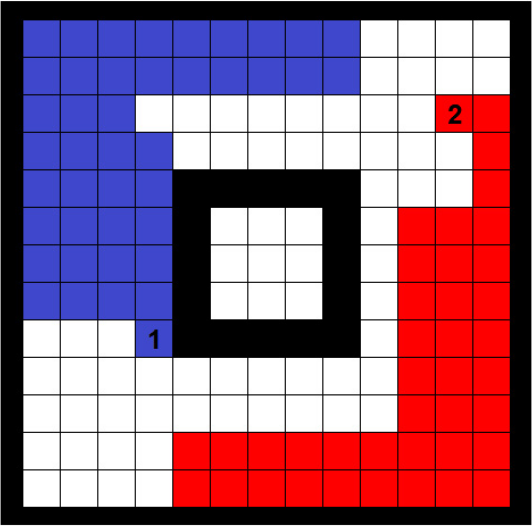
\includegraphics[width=4.6cm]{images/tron_field.png} \hspace{0.4cm} 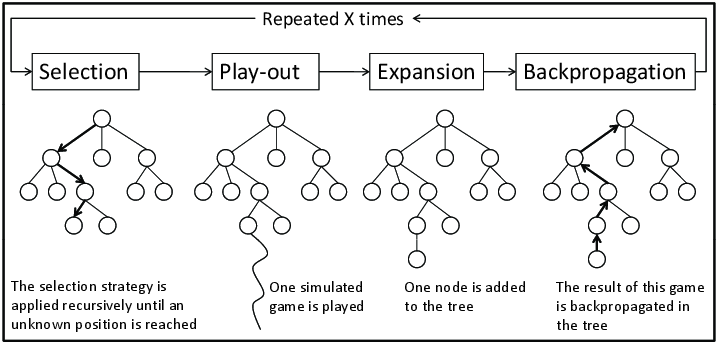
\includegraphics[width=9.8cm]{images/mcts_figure.png}
\caption{(Left) A game in Tron. 41 moves are already played. Player 1 started in the top left corner and Player 2 started in the bottom right corner.
 (Right) The four phases of the Monte Carlo Tree Search. \label{fig:tron-mcts}}
\end{center}
\end{figure}


\subsection{Simultaneous Move MCTS}

%In the following subsections, the adaptation of MCTS to Tron is described~\cite{teuling_tron}. In particular how the simultaneous moves of the game are handled and which heuristic knowledge of the game of Tron can be used to increase the performance of the MCTS.

%\subsubsection*{Modeling Simultaneous Move Games}

%\label{subsec:sim_moves}
Standard MCTS applies to sequential turned-based games. However, in some games moves are chosen simultaneously. 
There are two models to handle the simultaneous moves that occur in Tron. 

The first model, used to implement Sequential UCT, ignores the presence of simultaneous moves and treats the game as a sequential turn-based game inside the search tree. 
We call this the {\it sequential tree model}. 
In practice, this worked well in Tron~\cite{tron_cig,teuling_tron}, except it clearly favours one player which is especially problematic when players are close to each other. 
%Therefore, in our version of Tron we add an exception to the expansion phase. If the first player moves to a position that the second player can also move to, the opponent is still able to move there to achieve a draw rather than a loss~\cite{teuling_tron}. 
In this model, the game is sequential inside the search tree, until a leaf node is reached. The play-outs are then simulated as a simultaneous game~\cite{teuling_tron}. 
In this paper, the player running the search always moves first. 

The second model, used to implement simultaneous move MCTS, stores a matrix at each node. 
We call this the {\it stacked matrix model}.
Each cell of the matrix corresponds to a joint move, \ie a move chosen by both players simultaneously, and a corresponding child node (successor state). 
This is a more accurate representation of the underlying game since players are not able to base their current decision after having seen the other player's current move choice. 
This is the model used in~\cite{cig_paper} and \cite{mcts_goofspiel}.

%A novel contribution of this paper is the comparison of MCTS applied in these two different models. 

\section{Tron \& MCTS}
\label{sec:tron_specific_mcts}

%\label{sec:tron}
%The game of Tron, also known as Light-Cycle Racing, originates from the movie Tron released in 1982. The game is played in a grid like environment, where motorcycles can only drive on the grid, i.e. only drive forward or make 90 degree turns. In addition, the motorcycles create a wall behind them as they drive through the world.\\
%The game which is investigated in this paper,
Tron originates from the 1982 movie with the same name. It is a two-player game (See left part of Figure~\ref{fig:tron-mcts}) played on discrete grids possibly obstructed by walls. In addition, the maps are mostly symmetric so that none of the players have an advantage. Unlike sequential turn-taking games where payers play consecutively, at each step in Tron both players move simultaneously. The game is won if opponent crashes into a wall or moves off the board. If both players crash at the same turn into a wall, the game ends in a draw.
%To create an intelligent agent for this game is a challenging task, especially for the first moves, many computations have to be done in order to make a profound decision on which move to choose.




%\begin{figure}[b]
%\begin{center}
%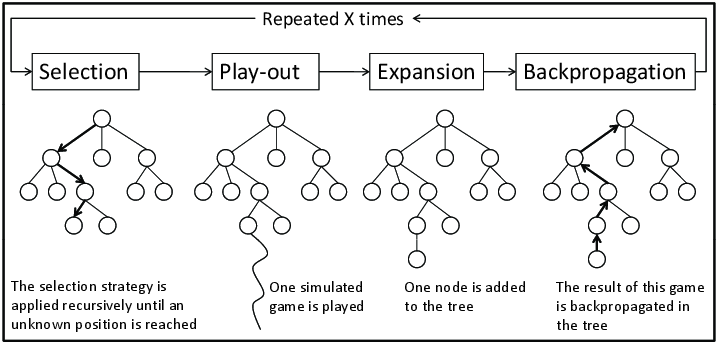
\includegraphics[width=0.9\textwidth]{images/mcts_figure.png}
%\caption{The four phases of the Monte Carlo Tree Search.\label{fig:mcts_figure}}
%\end{center}
%\end{figure}

% Removed the elaborate explanation of each phase for now. 


%\subsection{Heuristic Knowledge}
%\label{subsec:heuristic_knowledge}
%In the game of Tron, the MCTS can make use of some heuristic knowledge of the game to improve the play-out and expansion phase. 

%\subsubsection*{Space Estimation, Predictive Expansion Strategy, and Play-out Cut-Offs}

%Space Estimation is useful knowledge to have in the game of Tron. 
Tron is played in a grid-like environment and so often the two players become separated from each other. When this happens, each agent is essentially playing their own single-player game and the goal of the game becomes to outlast the opponent. Therefore the play-out can be prematurely terminated by counting the number of squares captured by each player and then assigning a win to whoever has claimed the most space. The problem is that some positions might not offer a way back and therefore become suicide moves. For that reason a greedy wall-following algorithm can be used, which tries to fill out the remaining space. When both players have filled their space, the moves which were made are counted and the player with the higher move count wins. This approach was proposed by Den Teuling~\cite{teuling_tron}. % and is used in Subsection~\ref{subsec:pes} and~\ref{subsec:play_out_cut_off}.

%\subsubsection*{Predictive Expansion Strategy}
%\label{subsec:pes}
%In the game of Tron, it is common that the players get separated from each other. 
Also, when players are separated, there is no need to let a play-out decide which player would win. Instead, it can be predicted by the Predictive Expansion Strategy (PES)~\cite{teuling_tron}. PES is used to avoid play-outs when they are not necessary. Each time the non-root player tries to expand a node, the PES checks whether the two players are separated from each other. If this is the case, space estimation is used to predict which player would win. Finally, the expanded node becomes a leaf node and no more play-outs have to be done when reaching this node again. 

%The saved time can be used for more simulations. 

%\subsubsection*{Play-out Cut-Off}
%\label{subsec:play_out_cut_off}

% ML: A lot of this is already said above. 
%During the play-out phase, the game will eventually end and a winner can be determined. Sometimes the outcome of the play-out could be predicted before the play-out is over. %This is useful, because this saves time, which can be used for more simulations~\cite{teuling_tron}. 
%One way to predict the outcome, is to check whether the two players are separated from each other. 
%If this is the case, the space estimation heuristic can be applied again and the winner can be determined. The result will be back propagated in a usual manner. Since computing whether both players are separated from each other takes a lot of time, this is only done every five moves during the play-out.

\section{Selection and Backpropagation Strategies}
\label{sec:selection_strategies}

%The default selection strategy is, as mentioned in Subsection~\ref{subsec:selection}, a random strategy, where each child node is selected in a random manner. 
%The default selection strategy is to choose a child node uniformly at random.
%This can be obviously improved by using heuristics and collected statistics. 
In the following subsections, different selection and update strategies for MCTS are introduced including deterministic strategies such as Sequential UCT and UCB1-Tuned, Decoupled UCT and Decoupled UCB1-Tuned, as well as stochastic strategies, which include Exp3 and Regret Matching. 

\subsection{Sequential UCT}
\label{subsec:uct}
The most common selection strategy is the Upper Confidence Bounds for Trees (UCT) \cite{kocsis}. The UCT strategy uses the Upper Confidence Bound (UCB1 \cite{auer_et_al}) algorithm. 
%If it is assumed that a sufficient number of play-outs (parameter $T$) have been made for a node
After each child has been at least selected once, UCB1 is used to select a child. This algorithm maintains a good balance between exploration and exploitation. UCB1 selects a child node $k$ from a set of nodes $K$, from parent node $j$ by using Equation~\ref{uct}:

\begin{equation}\label{uct}
  k = \argmax_{i \in K} \left\{ \bar{X}_{i} + C \sqrt{\frac{\ln (n_{j})}{n_{i}}} \right\},
\end{equation}
where $n_{i}$ is the number of visits of child node $i$ and $\bar{X}_{i}$ is the sample mean of the rewards of child node $i$. 
The parameter $C$ is usually tuned to increase performance. Sequential UCT was first applied to Tron in~\cite{tron_cig}.

%For the game of Tron these are initially set~\cite{teuling_tron} to $T=30$ and $C=10$.
%\subsection{Sequential UCB1-Tuned}
%\label{subsec:ucb1_tuned}

An enhancement to the UCT selection strategy can be made by replacing the parameter $C$ by an upper bound of the variance of the rewards \cite{cig_paper}. This is either $\frac{1}{4}$, which is an upper bound of the variance of a \emph{Bernoulli} random variable, or an upper confidence bound computed using Equation~\ref{ucb1tuned} which has the parameters the parent node $j$ and some child node $i$.
This variant is referred to as UCB1-Tuned~\cite{auer_et_al}.
Then, a child node $k$ is selected from parent node $j$:

\begin{equation}\label{ucb1tuned}
k = \argmax_{i \in K} \left\{ \bar{X}_{i} + \sqrt{\frac{\min(\frac{1}{4},\mbox{Var}_{UCB1}(j,i)) \ln (n_{j})}{n_{i}}} \right\}, 
\mbox{ \hspace{0.1cm} } 
\mbox{Var}_{UCB1}(j,i)=\bar{s} ^2_{k}+\sqrt{\frac{2 \ln (n_{j})}{n_{i}}},
\end{equation}
where $\bar{s} ^2_{k}$ is the sample variance of the observed rewards for child node $k$. 

%\begin{equation}\label{ucb1tuned}
%\end{equation}

\subsection{Decoupled UCT}
\label{subsec:duct}

Unlike standard sequential UCT and UCB1-Tuned used in the sequential tree model, Decoupled UCT (DUCT) applies UCB1 selection in the stacked matrix model for each player separately.
%In fact, the representation of a node is changed. \
In DUCT a node stores the both moves, the one from Player 1 and from Player 2. 
UCB1 selects a move twice, once for each player, and independently of the other player's choice.  
To better illustrate the difference between these two concepts, see Figure~\ref{fig:suct_vs_duct}. In the left figure, the sequential tree model is shown. In the right figure, each node contains two moves, one belonging to Player 1 and one to Player 2. These combinations are called {\it joint moves}. Because each level in the search tree represents now one step in the game, the branching factor is nine instead of three.

When selecting a child node, DUCT applies the default UCB1 algorithm which was described in Equation~\ref{uct} with the statistics from each player's perspective independently. After a move is selected Player 1, the selection process is repeated for Player 2 (without knowledge of the choice made by Player 1) using the statistics from Player 2's perspective. These two moves are combined to form a joint move.
%Afterwards it combines the result of Player 2, for instance the move which represents the move ``right'' and chooses the child node which contains the joint-action [L,R].\\
The final move to be played, after many simulations, can be selected in two different ways. The first, DUCT(max), selects the move with the most visits. 
DUCT(mix) normalizes the visit counts and samples a move according to this distribution, \ie using a mixed strategy \cite{mcts_goofspiel}. 
%A mixed strategy is constructed such that the probability of each action being played corresponds to the value of the normalized values.
DUCT(max) and DUCT(mix) were first used in general game-playing programs~\cite{finnson_master,Shafiei09}.

\begin{figure}
\begin{center}
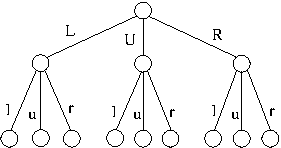
\includegraphics[width=6cm]{seq-model.pdf}~~~~~~~~~~~~~~~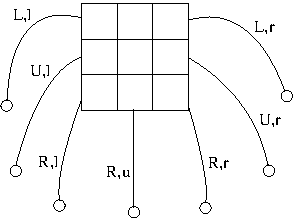
\includegraphics[width=4.4cm]{mat-model.pdf}
\caption{(Left) The sequential tree model. Each node represent the child node of the corresponding move. The first level represents Player 1 moves (L, U, and R) and the second level represents Player 2 moves (l, u, r). 
(Right) The stacked matrix model. Each joint move leads to a child node from a combination of moves for Player 1 and Player 2 (only 7 of the 9 joint moves are shown).
\label{fig:suct_vs_duct}}
\end{center}
\end{figure}

%\begin{figure}
%\begin{center}
%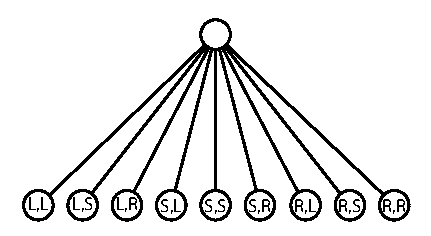
\includegraphics[width=8.5cm]{images/graph_dec_uct.pdf}
%\caption{A tree resembling the structure of decoupled MCTS. Each node represents a joint-action consisting of two moves, one for Player 1 and one for Player 2. L,S and R represents the different moves a player can make. L=Left, S=Straight and R=Right. Hence, (L,S) stands for Player1=Left and Player2=Right.\label{fig:graph_duct}}
%\end{center}
%\end{figure}

%\subsection{Decoupled UCB1-Tuned}
%\label{subsec:decoupled_ucb1_tuned}

Just as an enhancement can be made by replacing the parameter $C$ by an upper bound of the variance of the rewards in UCT, it can also be made to DUCT. Each time a node is selected and a joint move is chosen, Equation~\ref{ucb1tuned} is used. We refer to this variant as Decoupled UCB1-Tuned (DUCB1T).

\subsection{Exp3}
\label{subsec:exp3}

To this point, except for the final move selection in DUCT(mix), policies for selecting moves have been deterministic. Exp3~\cite{Exp3} belongs to the group of stochastic selection strategies, which means that there is a random factor involved and instead moves are sampled according to some probability distribution. %that we cannot tell deterministically beforehand which action is going to be chosen. 
Exp3, as DUCT, always uses the stacked matrix model and hence selects joint move.
Exp3 stores a list of estimated sums of rewards $\hat{X}_{a^{p}_{k}}$, where $a^{p}_{k}$ refers to player $p$'s move $k$. From the list of payoffs, a policy $P$ is created. The probability of choosing move $a^{p}_{k}$ of policy $P$ is shown in Equation~\ref{exp3_equations}, 

\begin{equation}\label{exp3_equations}
%P_{a^{p}_{k}}=\frac{e^{\hat{X}_{a^{p}_{k}}}}{\sum\limits_{i \in K_{p}}e^{\hat{X}_{a^{p}_{i}}}},
P_{a^{p}_{k}}=\frac{e^{\eta\omega(a^{p}_{k})}}{\sum\limits_{i \in A_{p}}e^{\eta\omega(a^{p}_{i})}}, 
\mbox{\hspace{1cm}}
\hat{X}_{a^{p}_{k}} = \hat{X}_{a^{p}_{k}} + \frac{r^{p}_{a_{k_{1}},a_{k_{2}}}}{\sigma_{a^{p}_{k}}},
\end{equation}
where $K_{p}$ is the set of moves from player $p$, $\omega$ can be scaled by some constant $\eta$, $r^{p}_{a_{k_{1}},a_{k_{2}}}$ is the reward of the play-out when Player 1 player chose move $k_{1}$ and Player 2 chose move $k_{2}$ and is give in respect to player $p$.
As in~\cite{mcts_goofspiel}, we set $\eta = \gamma / |K_p|$. 
%For simplicity, $\eta=1$ is chosen. 
In standard Exp3, $\omega(a^p_k) = \hat{X}_{a^p_k}$, but in practice we use $\omega(a^{p}_{k} ) = \hat{X}_{a^{p}_{k}} - \argmax_{i \in K_{p}}\hat{X}_{a^{p}_{i}}$ since it is equivalent and more numerically stable~\cite{mcts_goofspiel}.
The move selected is then sampled from the mixed strategy where move $a^p_k$ is selected with probability $\sigma_{a^{p}_{k}}=(1-\gamma)  P_{a^{p}_{k}} + \frac{\gamma}{|K_{p}|}$.

%Since Equation~\ref{exp3_policy} leads to numerical instability, Equations~\ref{exp3_policy_new} and~\ref{exp3_policy_weight} are used instead. From this policy, a probability $\sigma_{a^{p}_{k}}$ is computed (See Equation~\ref{exp3_distribution}) from which a mixed strategy is played. 
%Otherwise $\eta$ can be tuned to increase the performance of Exp3.

%\begin{equation}\label{exp3_policy_weight}
%\omega(a^{p}_{k})=\hat{X}_{a^{p}_{k}}-argmax_{i \in A_{p}}\hat{X}_{a^{p}_{i}}
%\end{equation}

%\begin{equation}\label{exp3_distribution}
%\sigma_{a^{p}_{k}}=(1-\gamma) \times P^{new}_{a^{p}_{k}} + \frac{\gamma}{|A_{p}|}
%\end{equation}
%\begin{equation}\label{exp3_update}
%\end{equation}

Parameter $\gamma$ can be optimized by tuning it. The update of $\hat{X}_{p}(a_{n})$ after selecting a joint move $(a_{1},a_{2})$, by using the probability $\sigma_{i}(a_{j})$, which returned some simulation result of a play-out $r^{p}_{a_{k_{1}},a_{k_{2}}}$ is given in Equation~\ref{exp3_equations}.
As in DUCT(mix), the final move is sampled from the normalized visit count distribution.

%The final move is chosen in the same way as it was in DUCT(mix).


\subsection{Regret Matching}
\label{subsec:rm}
Regret Matching (RM)~\cite{Hart00}, as Exp3 and DUCT, selects always joint move. Opposed to the other strategies, Regret Matching stores a matrix $M$ with the estimated mean of the rewards (See Equation~\ref{rm_equations}, where $\bar{X}_{m,n}$ is the mean of the rewards for Player 1 when the joint move $(a_{1}=m,a_{2}=n)$ was selected).

\begin{equation}
\label{rm_equations}
M = 
\begin{bmatrix}
\bar{X}_{1,1} && \bar{X}_{2,1} && \bar{X}_{3,1} \\
\bar{X}_{1,2} && \bar{X}_{2,2} && \bar{X}_{3,2} \\
\bar{X}_{1,3} && \bar{X}_{2,3} && \bar{X}_{3,3}
\end{bmatrix}
\mbox{ \hspace{1cm} }
\begin{array}{c}
\forall a^{1}_{i} \in K_{1}, R_{a^{1}_{i}} = R_{a^{1}_{i}} + (reward^1_{i,n} - r^{1}_{a_{m},a_{n}})\\
\forall a^{2}_{i} \in K_{2}, R_{a^{2}_{i}} = R_{a^{2}_{i}} + (reward^2_{m,i} - r^{2}_{a_{m},a_{n}})
\end{array}
\end{equation}

Additional to matrix $M$, two lists are stored which keep track of the cumulative regret for not taking move $a^p_k$, denoted $R_{a^{p}_{k}}$.
%$is the cumulative regret of player $p$ not having taken action $k$). 
The regret is a value, which indicates how much the player regrets not having played this move. 
%This is the fundamental idea of this selection strategy. 
%With the help of the two lists containing the cumulative regret, 
A policy $P$ is then constructed created by normalizing over the positive cumulative regrets (\eg if the regrets are $R_{a^{1}_{1}} = 8.0$, $R_{a^{1}_{2}} = 5.0$ and $R_{a^{1}_{3}} = -4.0$, then the policy is the probability distribution $(\frac{8}{13}, \frac{5}{13}, 0)$. 
As in Exp3, the selected move is sampled from $\sigma_{a^{p}_{k}}=(1-\gamma) P_{a^{p}_{k}} + \frac{\gamma}{|K_{p}|}$. 
where the variable $\gamma$ can be tuned to increase performance as in Exp3.

%these policies are used to compute a probability from which a mixed strategy is played (See Equation~\ref{regret_eq}. 

%\begin{equation}\label{regret_eq}
%\sigma_{a^{p}_{k}}=(1-\gamma) P_{a^{p}_{k}} + \frac{\gamma}{|A_{p}|}
%\end{equation}

Initially, all values in matrix $M$ and all values in the regret lists are set to zero. After the play-out is finished and the result ($r^{p}_{a_{m},a_{n}}$) for player $p$ gets back propagated, the cumulative reward values for each cell are updated using $X_{m,n} = X_{m,n} + r^{p}_{a^{1}_{m},a^{2}_{n}}$ and the regret values are updated using the right side of Equation~\ref{rm_equations},
where $reward^p_{m',n'} = r^p_{a_m,a_n}$ if $(m',n') = (m,n)$ or $\bar{X}_{m,n}$ otherwise.
The final move is selected using the average of all the mixed strategies used over all simulations as described in~\cite{mcts_goofspiel}. 
%in DUCT(mix) and Exp3 by sampling from the mixed strategy of normalized visit counts. 
%The final move is selected as in DUCT(mix) and Exp3 by sampling from the mixed strategy of normalized visit counts. 

%\begin{equation}\label{update_matrix}
%\begin{align}
%X_{m,n} = X_{m,n} + r^{p}_{a^{1}_{m},a^{2}_{n}}
%\end{align}
%\end{equation}

%\begin{equation}\label{update_regret}
%\begin{align}
%\end{align}
%\end{equation}


\section{Experiments}
\label{sec:experiments}

In this section the different selection and backpropagation strategies are evaluated. 
%Because the framework, which was implemented by Teuling~\cite{teuling_tron}, used for this experiments is based on sequential UCT, DUCT, Exp3 and Regret Matching were not optimally implemented. 
%Therefore it would be an unfair comparison, if all agents would have the same thinking time. 
In order to make it a fair comparison between the two search tree models using a common implementation, each agent is allowed to simulate a fixed number of simulations (100,000) which took roughly one second on modern hardware. 

%In the case of this experiment the number is set to 100,000. 
The experiments are run on four different boards, three with obstacles (see Figure~\ref{fig:boards-example}) and an empty board (d)), all with dimensions of $13 \times 13$. On each board 500 games are played per player matchup.
%to assure that none of the agents are benefiting from starting in a certain position. 
The play-out strategy, which is used in all experiments, is the random strategy with play-out cut-offs enhancement mentioned in Section~\ref{sec:tron_specific_mcts}. 
However, to avoid slowing down playouts too much, they are only applied every 10 steps. 
The expansion strategy uses the predictive expansion strategy.

%Some parameters are tuned in Subsection~\ref{subsec:parameter_tuning} and the several selection strategies introduced in this paper, are tested against each other in a round-robin tournament in Subsection~\ref{subsec:round_robin}. In addition another round-robin tournament is conducted on a smaller $6 \times 6$ board to see how the results differ from the ones conducted in the round-robin tournament on the large boards.

\begin{figure}
\centering 
\begin{subfigure}[c]{0.5\textwidth}
\centering
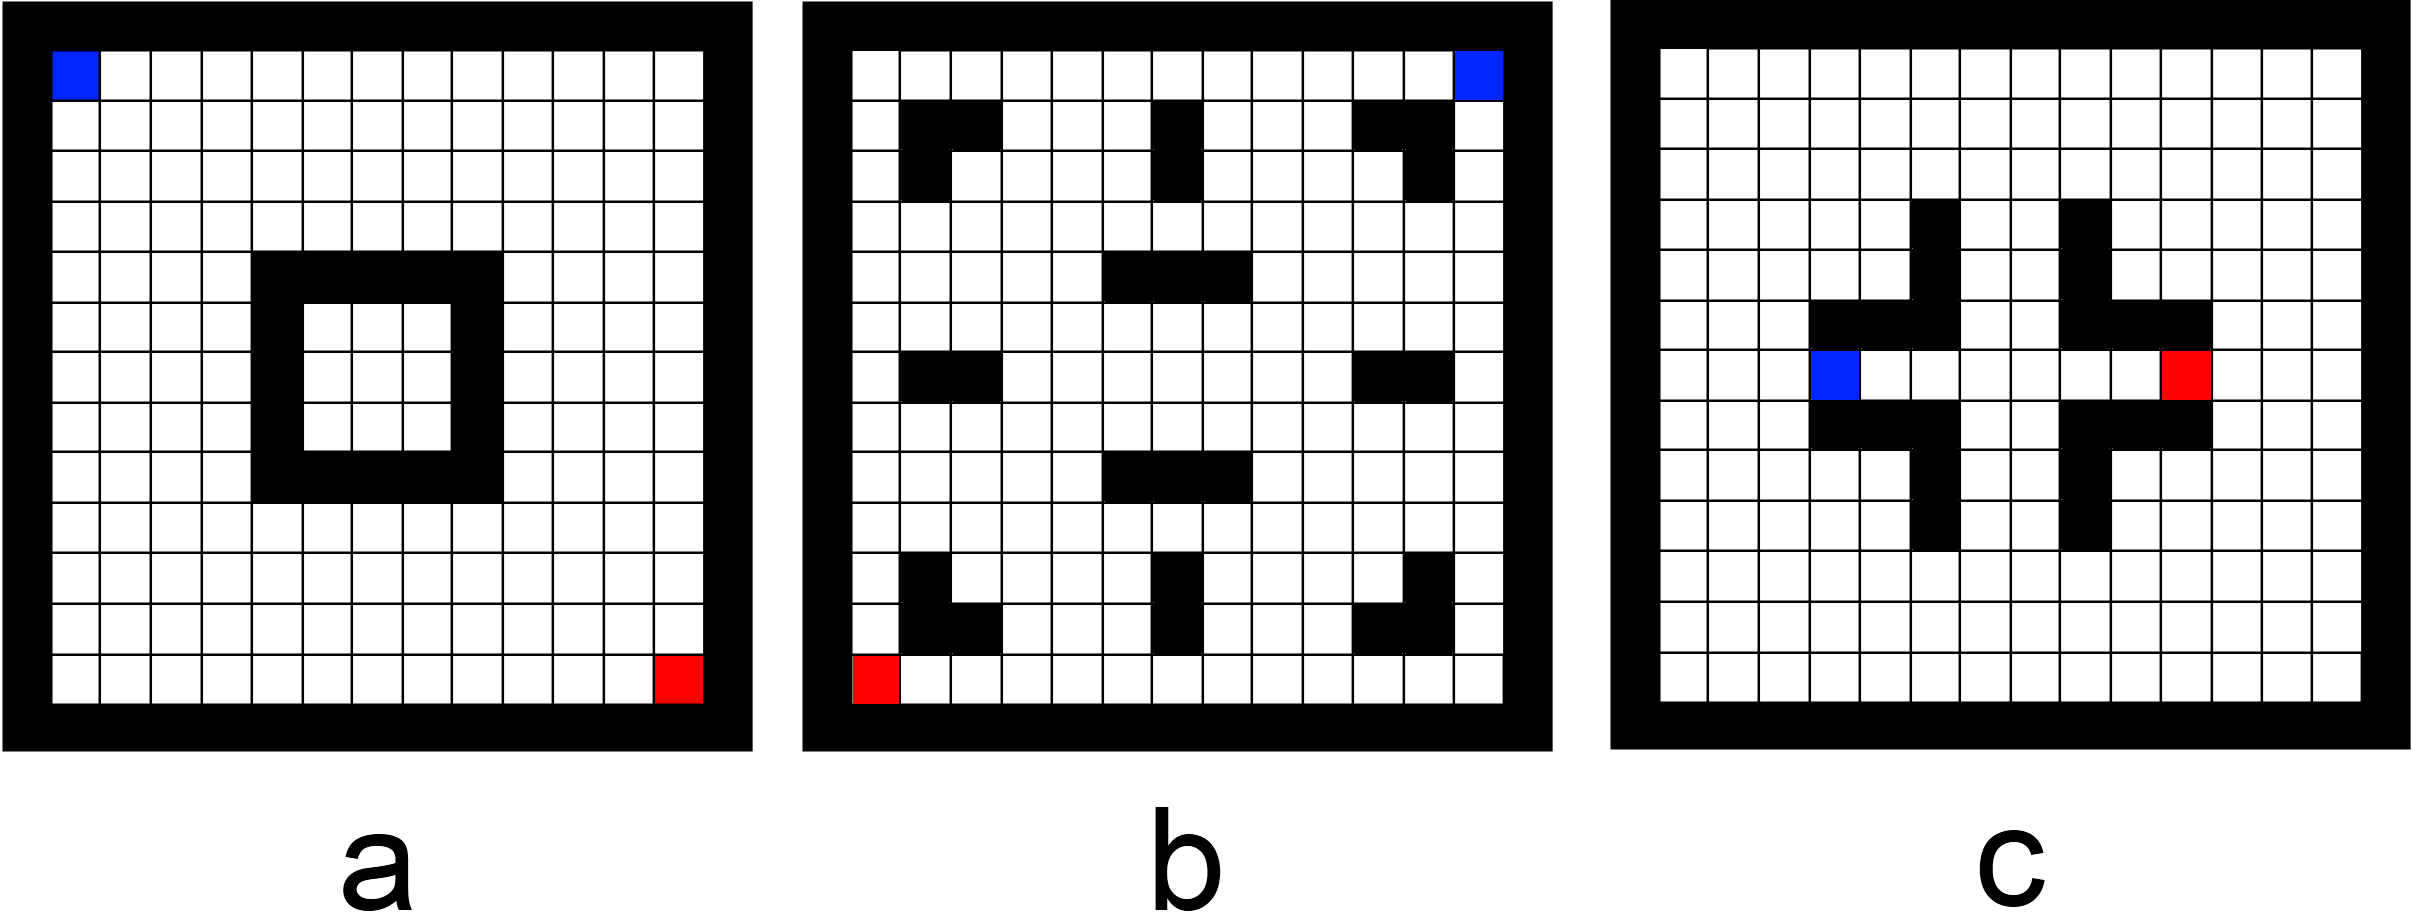
\includegraphics[width=\textwidth]{images/boards.png} 
%\caption{Four different boards are used for the experiments in the round-robin tournament. a,b and c, as well as the empty board, d, of the same size.\label{fig:ex_boards}}
\end{subfigure}
~~~~~~~~~~~~~~
\begin{subfigure}[c]{0.29\textwidth}
\centering
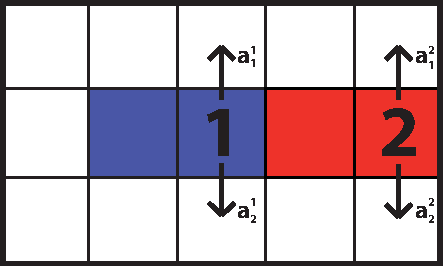
\includegraphics[width=\textwidth]{images/stochastic.pdf}
\end{subfigure}
%\begin{table}[b]
\caption{Left: Different boards are used for the experiments in the round-robin tournament. Right: A situation whose optimal strategies require mixing with probability distribution $(0.5, 0.5)$. \label{fig:boards-example}}
\end{figure}

\begin{table}[t]\scriptsize
\centering
\begin{tabular}{|c||c|c|c|c|c|c|c|c|}
									\hline
  Board a 		& UCT 	& UCB1T		& DUCT(max)	& DUCT(mix)	& DUCB1T(max)	& DUCB1T(mix)	& Exp3	& RM				\\ 	\hline\hline
   UCT &    - & 44\% & 51\% & 58\% & 40\% & 45\% & 53\% & 41\% \\ \hline 
 UCB1T & 56\% &    - & 67\% & 68\% & 48\% & 55\% & 60\% & 51\% \\ \hline 
   DUCT(max) & 49\% & 33\% &    - & 53\% & 28\% & 32\% & 73\% & 35\% \\ \hline 
   DUCT(mix) & 42\% & 32\% & 47\% &    - & 28\% & 33\% & 58\% & 35\% \\ \hline 
 DUCB1T(max) & 60\% & 52\% & 72\% & 72\% &    - & 59\% & 78\% & 63\% \\ \hline 
 DUCB1T(mix) & 55\% & 45\% & 68\% & 67\% & 41\% &    - & 67\% & 48\% \\ \hline 
      Exp3 & 47\% & 40\% & 27\% & 42\% & 22\% & 33\% &    - & 33\% \\ \hline 
        RM & 59\% & 49\% & 65\% & 65\% & 37\% & 52\% & 67\% &    - \\ \hline 
%UCT 			&  -	& 61\%		& 51\% 		& 54\%		& 53\%		& 67\%		& 65\%	& 62\%				\\ 	\hline
%  UCB1T 		& 39\% 	& - 		& 53\%		& 61\%		& 52\%		& 65\%		& 66\%	& 61\%				\\ 	\hline
%  DUCT(max) 		& 49\% 	& 47\%		& -		& 67\%		& 43\%		& 62\%		& 63\%	& 67\%				\\ 	\hline
%  DUCT(mix) 		& 46\% 	& 39\% 		& 33\%		& -		& 37\%		& 48\%		& 53\%	& 51\%				\\ 	\hline
%  DUCB1T(max)	 	& 47\% 	& 48\% 		& 57\%		& 63\%		& -		& 61\%		& 64\%	& 69\%				\\ 	\hline
%  DUCB1T(mix)	 	& 33\% 	& 35\% 		& 38\%		& 52\%		& 39\%		& -		& 54\%	& 51\%				\\ 	\hline
%  Exp3 			& 35\% 	& 34\% 		& 37\%		& 47\%		& 36\%		& 46\%		& -	& 51\%				\\ 	\hline
%  RM		 	& 38\%	& 39\% 		& 33\%		& 49\%		& 31\%		& 49\%		& 49\%	& -				\\ 	\hline
\end{tabular}
\begin{tabular}{|c||c|c|c|c|c|c|c|c|}
									\hline
  Board b 		& UCT 	& UCB1T		& DUCT(max)	& DUCT(mix)	& DUCB1T(max)	& DUCB1T(mix)	& Exp3	& RM				\\ 	\hline\hline
   UCT &    - & 50\% & 51\% & 57\% & 49\% & 51\% & 72\% & 50\% \\ \hline 
 UCB1T & 50\% &    - & 53\% & 65\% & 50\% & 52\% & 70\% & 56\% \\ \hline 
   DUCT(max) & 49\% & 47\% &    - & 63\% & 41\% & 46\% & 79\% & 52\% \\ \hline 
   DUCT(mix) & 43\% & 35\% & 37\% &    - & 24\% & 32\% & 70\% & 38\% \\ \hline 
 DUCB1T(max) & 51\% & 50\% & 59\% & 76\% &    - & 55\% & 83\% & 62\% \\ \hline 
 DUCB1T(mix) & 49\% & 48\% & 54\% & 68\% & 45\% &    - & 80\% & 54\% \\ \hline 
      Exp3 & 28\% & 30\% & 21\% & 30\% & 17\% & 20\% &    - & 23\% \\ \hline 
        RM & 50\% & 44\% & 48\% & 62\% & 38\% & 46\% & 77\% &    - \\ \hline 
%  UCT 			&  -	& 47\%		& 49\%		& 57\%		& 51\%		& 61\%		& 61\%	& 59\%				\\ 	\hline
%  UCB1T 		& 53\% 	& - 		& 51\%		& 54\%		& 49\%		& 65\%		& 64\%	& 57\%				\\ 	\hline
%  DUCT(max) 		& 51\% 	& 49\% 		& -		& 54\%		& 51\%		& 58\%		& 54\%	& 52\%				\\ 	\hline
%  DUCT(mix) 		& 43\%	& 46\% 		& 46\%		& -		& 41\%		& 52\%		& 49\%	& 46\%				\\ 	\hline
%  DUCB1T(max)	 	& 49\% 	& 51\% 		& 49\%		& 59\%		& -		& 68\%		& 62\%	& 65\%				\\ 	\hline
%  DUCB1T(mix)	 	& 39\% 	& 35\% 		& 42\%		& 48\%		& 32\%		& -		& 57\%	& 52\%				\\ 	\hline
%  Exp3 			& 39\% 	& 36\% 		& 46\%		& 51\%		& 38\%		& 43\%		& -	& 57\%				\\ 	\hline
%  RM 			& 41\% 	& 43\% 		& 48\%		& 54\%		& 35\%		& 48\%		& 43\%	& -				\\ 	\hline
\end{tabular}
\begin{tabular}{|c||c|c|c|c|c|c|c|c|}
									\hline
  Board c 		& UCT 	& UCB1T		& DUCT(max)	& DUCT(mix)	& DUCB1T(max)	& DUCB1T(mix)	& Exp3	& RM				\\ 	\hline\hline
   UCT &    - & 64\% & 57\% & 56\% & 46\% & 54\% & 56\% & 50\% \\ \hline 
 UCB1T & 36\% &    - & 44\% & 60\% & 42\% & 47\% & 62\% & 52\% \\ \hline 
   DUCT(max) & 43\% & 56\% &    - & 55\% & 42\% & 49\% & 57\% & 41\% \\ \hline 
   DUCT(mix) & 44\% & 40\% & 45\% &    - & 28\% & 36\% & 57\% & 49\% \\ \hline 
 DUCB1T(max) & 54\% & 58\% & 58\% & 72\% &    - & 60\% & 75\% & 61\% \\ \hline 
 DUCB1T(mix) & 46\% & 53\% & 51\% & 64\% & 40\% &    - & 64\% & 55\% \\ \hline 
      Exp3 & 44\% & 38\% & 43\% & 43\% & 25\% & 36\% &    - & 36\% \\ \hline 
        RM & 50\% & 48\% & 59\% & 51\% & 39\% & 45\% & 64\% &    - \\ \hline 
%  UCT 			&  -	& 37\% 		& 81\%		& 89\%		& 84\%		& 96\%		& 71\%	& 72\%				\\ 	\hline
%  UCB1T 		& 63\% 	& - 		& 79\%		& 71\%		& 88\%		& 89\%		& 73\%	& 70\%				\\ 	\hline
%  DUCT(max) 		& 19\% 	& 21\% 		& -		& 58\%		& 41\%		& 52\%		& 69\%	& 61\%				\\ 	\hline
%  DUCT(mix) 		& 11\% 	& 29\% 		& 42\%		& -		& 39\%		& 49\%		& 51\%	& 51\%				\\ 	\hline
%  DUCB1T(max)	 	& 16\% 	& 12\% 		& 59\%		& 61\%		& -		& 59\%		& 68\%	& 64\%				\\ 	\hline
%  DUCB1T(mix)	 	& 4\%  	& 11\% 		& 48\%		& 51\%		& 41\%		& -		& 50\%	& 58\%				\\ 	\hline
%  Exp3 			& 29\% 	& 27\% 		& 31\%		& 49\%		& 32\%		& 50\%		& -	& 49\%				\\ 	\hline
%  RM 			& 28\% 	& 30\% 		& 39\%		& 49\%		& 36\%		& 42\%		& 51\%	& -				\\ 	\hline
\end{tabular}
\begin{tabular}{|c||c|c|c|c|c|c|c|c|}
									\hline
  Board d 		& UCT 	& UCB1T		& DUCT(max)	& DUCT(mix)	& DUCB1T(max)	& DUCB1T(mix)	& Exp3	& RM				\\ 	\hline\hline
   UCT &    - & 46\% & 47\% & 57\% & 44\% & 48\% & 52\% & 48\% \\ \hline 
 UCB1T & 54\% &    - & 51\% & 60\% & 50\% & 52\% & 57\% & 53\% \\ \hline 
   DUCT(max) & 53\% & 49\% &    - & 64\% & 35\% & 45\% & 58\% & 48\% \\ \hline 
   DUCT(mix) & 43\% & 40\% & 36\% &    - & 29\% & 35\% & 39\% & 30\% \\ \hline 
 DUCB1T(max) & 56\% & 50\% & 65\% & 71\% &    - & 55\% & 65\% & 56\% \\ \hline 
 DUCB1T(mix) & 52\% & 48\% & 55\% & 65\% & 45\% &    - & 56\% & 50\% \\ \hline 
      Exp3 & 48\% & 43\% & 42\% & 61\% & 35\% & 44\% &    - & 42\% \\ \hline 
        RM & 52\% & 47\% & 52\% & 70\% & 44\% & 50\% & 58\% &    - \\ \hline 
%  UCT 			&  -	& 52\%		& 48\%		& 51\%		& 50\%		& 64\%		& 67\%	& 65\%				\\ 	\hline
%  UCB1T 		& 48\% 	& - 		& 45\%		& 57\%		& 53\%		& 67\%		& 59\%	& 67\%				\\ 	\hline
%  DUCT(max) 		& 52\% 	& 55\% 		& -		& 60\%		& 49\%		& 61\%		& 59\%	& 62\%				\\ 	\hline
%  DUCT(mix) 		& 49\% 	& 43\% 		& 40\%		& -		& 41\%		& 55\%		& 50\%	& 49\%				\\ 	\hline
%  DUCB1T(max)	 	& 50\% 	& 47\% 		& 51\%		& 59\%		& -		& 57\%		& 64\%	& 68\%				\\ 	\hline
%  DUCB1T(mix)	 	& 36\% 	& 33\% 		& 39\%		& 45\%		& 43\%		& -		& 51\%	& 49\%				\\ 	\hline
%  Exp3 			& 33\% 	& 41\% 		& 41\%		& 50\%		& 36\%		& 49\%		& -	& 52\%				\\ 	\hline
%  RM 			& 35\% 	& 23\% 		& 38\%		& 51\%		& 32\%		& 51\%		& 48\%	& -				\\ 	\hline
\end{tabular}
%\caption{Results of the different selection strategies playing on Board a,b,c and d.}
\caption{Results of the different selection strategies playing on boards a, b, c and d. 
Each percentage refers to the win rate of the row player. \label{table:round_robin}}
%UCB1T=UCB1-Tuned, DUCB1T(max)=DUCB1-Tuned(max), DUCB1T(mix)=DUCB1-Tuned(mix), RM=Regret Matching;
\end{table}

\begin{table}[h!]\scriptsize
\centering
\begin{tabular}{|c||c|c|c|c|c|c|c|c|}
									\hline
  Total 	     	& UCT 	& UCB1T		& DUCT(max)	& DUCT(mix)	& DUCB1T(max)	& DUCB1T(mix)	& Exp3	& RM				\\ 	
  \hline
  \hline
   UCT &    - & 50\% & 51\% & 55\% & 46\% & 49\% & 57\% & 48\% \\ \hline 
 UCB1T & 50\% &    - & 53\% & 61\% & 48\% & 51\% & 60\% & 52\% \\ \hline 
   DUCT(max) & 49\% & 47\% &    - & 58\% & 39\% & 45\% & 63\% & 45\% \\ \hline 
   DUCT(mix) & 45\% & 39\% & 42\% &    - & 31\% & 36\% & 55\% & 40\% \\ \hline 
 DUCB1T(max) & 54\% & 52\% & 61\% & 69\% &    - & 56\% & 70\% & 59\% \\ \hline 
 DUCB1T(mix) & 51\% & 49\% & 55\% & 64\% & 44\% &    - & 64\% & 51\% \\ \hline 
      Exp3 & 43\% & 40\% & 37\% & 45\% & 30\% & 36\% &    - & 34\% \\ \hline 
        RM & 52\% & 48\% & 55\% & 60\% & 41\% & 49\% & 66\% &    - \\ \hline 
%  UCT 			    &  -	  & 49\%		& 57\%		  & 63\%		& 60\%		& 72\%		& 66\%	& 64\%				\\ 	\hline
%  UCB1T 		    & 51\% 	& - 		  & 57\%		  & 61\%		& 61\%		& 71\%		& 65\%	& 63\%				\\ 	\hline
%  DUCT(max) 		& 43\% 	& 43\% 		& -		      & 60\%		& 46\%		& 58\%		& 61\%	& 60\%				\\ 	\hline
%  DUCT(mix) 		& 37\% 	& 39\% 		& 40\%		  & -		    & 40\%		& 51\%		& 51\%	& 49\%				\\ 	\hline
%  DUCB1T(max)	 	& 40\% 	& 39\% 		& 54\%		  & 60\%		& -	     	& 61\%		& 65\%	& 67\%				\\ 	\hline
%  DUCB1T(mix)	 	& 18\% 	& 19\% 		& 42\%		  & 49\%		& 39\%		& -		    & 53\%	& 52\%				\\ 	\hline
%  Exp3 			    & 34\%	& 35\% 		& 39\%		  & 49\%		& 35\%		& 47\%		& -	    & 52\%				\\ 	\hline
%  RM		 	      & 36\% 	& 37\%		& 40\%		  & 51\%		& 33\%		& 48\%		& 48\%	& -				    \\ 	\hline
\end{tabular}
\caption{Overall results of the different selection strategies playing against each other over all boards.
Each percentage refers to the win rate of the row player. }
%Here, UCB1T=UCB1-Tuned, DUCB1T(max)=DUCB1-Tuned(max), DUCB1T(mix)=DUCB1-Tuned(mix), RM=Regret Matching}
\label{table:round_robin_total}
\end{table}

\begin{table}[h!]\scriptsize
\centering
\begin{tabular}{|c||c|c|c|c|c|c|c|c||c|}
									\hline
	6$\times$6 Board	& UCB1T 	& UCT		& DUCT(max)	& DUCB1T(max)	& DUCT(mix)	& DUCB1T(mix)	& Exp3 & RM & Total \\ \hline
   UCT &    - & 43\% & 50\% & 49\% & 50\% & 48\% & 50\% & 49\%       & 48.3 $\pm$ 0.4\% \\ \hline 
 UCB1T & 57\% &    - & 50\% & 51\% & 50\% & 50\% & 51\% & 50\%       & 51.2 $\pm$ 0.4\% \\ \hline 
   DUCT(max) & 50\% & 50\% &    - & 54\% & 50\% & 52\% & 51\% & 50\% & 51.0 $\pm$ 0.2\% \\ \hline 
   DUCT(mix) & 51\% & 49\% & 46\% &    - & 46\% & 47\% & 49\% & 48\% & 47.9 $\pm$ 0.5\% \\ \hline 
 DUCB1T(max) & 50\% & 50\% & 50\% & 54\% &    - & 51\% & 51\% & 50\% & 51.0 $\pm$ 0.2\% \\ \hline 
 DUCB1T(mix) & 52\% & 50\% & 48\% & 53\% & 49\% &    - & 51\% & 49\% & 50.5 $\pm$ 0.3\% \\ \hline 
      Exp3 & 50\% & 49\% & 49\% & 51\% & 49\% & 49\% &    - & 38\%   & 48.0 $\pm$ 0.4\% \\ \hline 
        RM & 51\% & 50\% & 50\% & 52\% & 50\% & 51\% & 62\% &    -   & 52.2 $\pm$ 0.4\% \\ \hline 
%	UCB1T							& -				& 52\%	& 59\%			& 62\%				& 59\%			& 62\%				& 57\%& 61\%	& 59 $\pm$ 2.57 \%		\\ \hline
%	UCT								& 48\%		& -			& 55\%			& 61\%				& 57\%			& 56\%				& 60\%& 59\%	& 57 $\pm$ 2.56 \%		\\ \hline
%	DUCT(max)					& 41\%		& 45\%	& -					& 48\%				& 56\%			& 56\%				& 54\%& 60\%	& 52 $\pm$ 2.62 \%		\\ \hline
%	DUCB1T(max)				& 38\%		& 39\%	& 52\%			& -						& 56\%			& 57\%				& 63\%& 61\%	& 52 $\pm$ 2.62 \%		\\ \hline
%	DUCT(mix)					& 41\%		& 43\%	& 44\%			& 44\%				& -					& 53\%				& 50\%& 49\%	& 47 $\pm$ 2.61 \%		\\ \hline
%	DUCB1T(mix)				& 38\%		& 44\%	& 44\%			& 43\%				& 43\%			& -						& 51\%& 54\%	& 46 $\pm$ 2.61 \%		\\ \hline
%	RM								& 43\%		& 40\%	& 46\%			& 37\%				& 50\%			& 46\%				& -		& 46\%	& 46 $\pm$ 2.61 \%		\\ \hline
%	Exp3							& 39\%		& 41\%	& 40\%			& 39\%				& 51\%			& 41\%				& 54\%& -			& 44 $\pm$ 2.60 \%		\\ \hline
\end{tabular}
\caption{Results of the different variants playing against each other on a $6\times6$ board. 
Each percentage refers to the win rate of the row player, and $\pm$ refers to 95\% confidence intervals.}
%\caption*{UCB1T=UCB1-Tuned, DUCB1T(max)=DUCB1-Tuned(max), DUCB1T(mix)=DUCB1-Tuned(mix), RM=Regret Matching}
\label{table:rr_small}
\end{table}


%\subsection{Parameter Tuning}
%\label{subsec:parameter_tuning}

Before running performance experiments, some parameters ($C$ in UCT, $\gamma$ in Exp3 and Regret Matching) are tuned. 
%This is done to assure that the different strategies perform optimally. 
As reference constants, values are used which were taken from different sources~\cite{teuling_tron,cig_paper}. Parameters $C$ and 
$\gamma \in [0,1]$ were tuned manually by playing several games against other variants. 
%After 10 games the value of the parameter $C$ was slightly increased or decreased, depending on how strong the UCT player played. 
%Starting with the reference constant, 120 games were played in order to find a value for $C$ which did not change significantly.
%The parameter $T$ used in UCT and UCB1-Tuned, which is the threshold before either UCT or UCB1-Tuned is applied as a selection strategy was tuned in the same way as the parameter $C$. This parameter tuning showed the same result as shown by Teuling~\cite{teuling_tron}, namely that the parameter $T$ does not influence the performance of UCT and UCB1-Tuned.\\
%The parameter $\gamma \in \[$ of Exp3 and Regret Matching was also tuned in the same way as the parameter $C$ with the only difference being that $\gamma$ must be in the interval of $[0,1]$.\\
The tuned values can be seen in Table~\ref{tbl:tunedvals}.
%The reference constants from previous work were $(C, T, \gamma(Exp3), \gamma(

\subsection{Round-Robin Tournaments}
\label{subsec:round_robin}

In this subsection, the performance of several players using different selection and backpropagation strategies are compared. 
This is done by playing matchups (of 500 games) of each player type against every other player type. 
Table~\ref{table:round_robin} presents the results of the games on all four maps and Table~\ref{table:round_robin_total} presents the average
performance of all players.
Table~\ref{tbl:overall-avgs} presents the average performance of each agent over boards a-d. 

%From this, we see that sequential UCT and UCB1-Tuned selection strategies perform best overall.
From this, we see that the UCB1-Tuned variants perform best overall, with the decoupled version 
winning significantly (8\%) more often than its next three competitors. 
Given that the top three players use UCB1-Tuned, including DUCB1T(mix), it appears that a better way of 
performing exploration has a bigger impact on performance than the choice of the game model 
(sequential versus stacked matrix).
%The round-robin tournament, in which every selection strategy played against each other, showed that the sequential UCB1-Tuned algorithm wins on average 63\% of its games and is therefore the winner of the tournament. 
%The max versions of the decoupled UCT and UCB1-Tuned strategy still perform reasonably well ($>50\%$). 
%All the other strategies, which include the mix versions of the decoupled UCT and UCB1-Tuned, as well as 
%Exp3 and Regret Matching, do not perform well overall ($<50\%$).
%Furthermore, the largest performance gap between sequential and simultaneous MCTS is in Board c. 
The relative rank of DUCB1T(max), DUCT(max), and Exp3 presented here on board (d) are consistent with 
previous results on the open map~\cite{cig_paper}. 
Sequential UCT performed relatively well, winning 51.39-54.32\% overall despite using a 
sequential model of the game. 
This could be because Sequential UCT learns to play safely since it chooses the move that minimizes over
the opponent's counter-moves. In fact, in the classic minimax setting the value computed in this model 
is a lower bound of the true optimal value~\cite{Bosansky13Using}. 

As in Goofspiel~\cite{mcts_goofspiel}, Regret Matching outperforms Exp3 and DUCT(mix). 
However unlike previous results in Goofspiel, Exp3 does not outperform 
DUCT(max). This may be because in Tron mistakes are not forgiving in the sense that it is easy to 
recognize and exploit suboptimal moves made by the opponent. 
Also, results of the algorithms vary from board to board, which is consistent with previous 
experiments in Tron~\cite{teuling_tron}. Board (b), for instance, can lead to many situations where 
a mistake made is particular difficult to recover from. In this situation, the deterministic strategies
tend to perform better since they avoid mistakes. 

%Generally the sequential strategies perform better than the decoupled strategies, which is especially visible on Board c (see Table~\ref{table:round_robin}), where the UCT and UCB1-Tuned only lost 4\%-19\% of its games against all DUCT strategies and only 28\%-29\% against Exp3 and Regret Matching, respectively. 
%Additionally, the deterministic selection strategies perform better than stochastic selection strategies on $16\times16$ boards, where all deterministic strategies win $>50\%$ and all stochastic win $<50\%$ of their matches. 

%sequential MCTS out performs the decoupled versions of MCTS.
%
The same round-robin tournament was repeated on a smaller ($6 \times 6$) board. 
From the results in Table~\ref{table:rr_small}, 
%generally the win rates get closer to 50\%.
%Since the board smaller, most of the variants can often compute the optimal choice. 
%we see that deterministic selection strategies are still doing better that stochastic 
%ones, but nonetheless perform better on the smaller board than on the larger board.
the round-robin tournament on the smaller $6 \times 6$ board the relative performance difference are less extreme, possibly
because each one is acting closer to optimally and there is less opportunity to make mistakes.
The deterministic strategies decrease and the performance of the stochastic strategies increase, with Regret Matching 
performing best in the small board, possibly because the stochastic strategies could be finding more situations where mixing 
among strategies is necessary. 
For example, in Figure~\ref{fig:boards-example} both players have two possible moves. If both players choose $a^{p}_{1}$ (``Left''), Player 1 wins and if both players choose $a^{p}_{2}$ (``Right''), Player 1 also wins. The optimal strategy for both players is to play with a mixed strategy, where each move is chosen with probability $0.5$. 

%\subsubsection*{Discussion}
%\label{subsec:discussion}

%The experiments revealed that the parameter $C$ of the UCT selection strategy was optimal at 13.2. 
%This value is higher than reported in the literature but in Tron, there are only 3 possible moves, therefore it may be beneficial to know where all three moves would lead us. 
%A high $C$ parameter ensures that the exploration of all nodes is given, which explains the result of the high $C$ parameter
%On the other hand, the tuning of $T$ showed little impact on overall performance. 
%of the UCT and UCB1-Tuned selection strategy was tuned. After some experiments, the tuning was stopped, because it did not seem to have much impact on the result of the selection strategies. 
%Therefore, 30 is still used for the parameter $T$. 
%The parameter $\gamma$ from the Exp3 and Regret Matching selection strategy was tuned to 0.39 and 0.31, respectively, to increase performance of those strategies.\\
%Already the selection strategies, which are deterministic, but only use a stochastic process to determine their final move, such as DUCT(mix) and DUCB1-Tuned(mix), perform way weaker than their counterparts DUCT(max) and DUCB1-Tuned(max).\\

%\begin{minipage}[c]{0.5\textwidth}
%\scriptsize
\begin{table}
\scriptsize
\begin{minipage}{.51\textwidth}
\begin{tabular}{|c||c|c|c|c|c|}
									\hline
 Variant	& a 		  & b 		  & c 		  & d 		  & Total 	\\ \hline
 DUCB1T(max) & 65\% & 62\% & 62\% & 59\% & 62.32 $\pm$ 0.56\% \\ \hline
 DUCB1T(mix) & 56\% & 57\% & 53\% & 53\% & 54.82 $\pm$ 0.61\% \\ \hline
 UCB1T & 58\% & 57\% & 49\% & 54\% & 54.32 $\pm$ 0.55\% \\ \hline
        RM & 56\% & 52\% & 51\% & 53\% & 53.13 $\pm$ 0.62\% \\ \hline
   UCT & 47\% & 54\% & 55\% & 49\% & 51.39 $\pm$ 0.55\% \\ \hline
   DUCT(max) & 43\% & 54\% & 49\% & 50\% & 49.05 $\pm$ 0.61\% \\ \hline
   DUCT(mix) & 39\% & 40\% & 43\% & 36\% & 39.51 $\pm$ 0.64\% \\ \hline
      Exp3 & 35\% & 24\% & 38\% & 45\% & 35.47 $\pm$ 0.61\% \\ \hline
%	UCB1-Tuned		      & 57\%	  & 58\%		& 78\%		& 58\%		& 63 $\pm$ 1.26\%		\\ \hline
%	UCT			            & 59\%		& 55\%		& 76\%		& 57\%		& 61 $\pm$ 1.28\%		\\ \hline
%	DUCB1-Tuned(max)	  & 58\%		& 58\%		& 48\%		& 57\%		& 55 $\pm$ 1.30\%		\\ \hline
%	DUCT(max)		        & 56\%		& 53\%		& 37\%		& 57\%		& 51 $\pm$ 1.31\%		\\ \hline
%	DUCT(mix)		        & 44\%		& 46\%		& 39\%		& 47\%		& 45 $\pm$ 1.30\%		\\ \hline
%	DUCB1-Tuned(mix)	  & 43\%		& 44\%		& 38\%		& 42\%		& 42 $\pm$ 1.29\%		\\ \hline
%	Exp3			          & 41\%		& 44\%		& 38\%		& 43\%		& 42 $\pm$ 1.29\%		\\ \hline
%	Regret Matching		  & 41\%		& 44\%		& 39\%		& 40\%		& 41 $\pm$ 1.28\%		\\ \hline
\end{tabular}
\caption{Results of the different variants played against each other. $\pm$ refers to 95\% confidence intervals. \label{tbl:overall-avgs}}
\end{minipage}
~~~~~
\begin{minipage}{.4\textwidth}
\scriptsize
%\caption{Results of the parameter-tuning of parameters $C$ and $T$ from the UCT Algorithm and from the parameter $\gamma$ of the Exp3 algorithm}
\begin{tabular}{|c||c|c|}
							\hline
Parameter			& Reference constant(s)                             & Tuned value	\\ \hline\hline
    $C$				& $10,3.52$ from~\cite{teuling_tron,cig_paper}	& $1.5$		\\ \hline
%$T$				& 30~\cite{teuling_tron}	& 30		\\ \hline
$\gamma$(Exp3) & 0.36~\cite{cig_paper}		& 0.3		\\ \hline
$\gamma$(Regret Matching)	& 0.025~\cite{mcts_goofspiel}				& 0.3		\\ \hline
\end{tabular}
%\label{table:parameter_tuning}
%\end{table}
\caption{Tuned parameter values. \label{tbl:tunedvals} }
\end{minipage}
\end{table}

\section{Conclusion and Future Research}
\label{sec:conclusion}

In this paper, several selection and backpropagation strategies were introduced for MCTS in Tron.
%including Sequential and Decoupled UCT, Sequential and Decoupled UCB1-Tuned, Exp3 and Regret Matching. 
The performance of these variants were tested in the game of Tron on different boards.
Overall, the round-robin tournament showed that the UCB1-Tuned variants perform best. % in the game of Tron. 
Furthermore the experiments showed that deterministic strategies perform generally better than the stochastic strategies in Tron.
The experiments also suggest that the layout of the board can influence the performance of a search algorithm.

For future research, we aim to do more experiments with different boards. 
%in order to determine why some boards (as Board c) create more difficulties for the decoupled strategies.\\
%In addition, the selection strategy Exp3 can be enhanced by tuning parameter $\eta$.
In addition, a hybrid selection strategy could be tested which uses a deterministic strategy if both players are far away from each other and a stochastic one as soon as both players come fairly close to each other. 
%This hybrid selection strategy would indicate, if the assumption made in this paper, that stochastic strategies perform better when both players are close to each other, is correct.

\vspace{0.2cm}
\noindent {\bf Acknowledgements} {\small This work is partially funded by MARBLE: Maastricht
Research Based Learning and the Netherlands Organisation
for Scientific Research (NWO) in the framework of the project
Go4Nature, grant number 612.000.938. }

\vspace{-0.5cm}
\bibliographystyle{plain}
\bibliography{sm-tron}



\end{document}








